% ---------------------------------------------------------------- cover -----
\thispagestyle{empty}
\begin{tikzpicture}[remember picture, overlay]
  \node[inner sep=0pt, anchor=north west] at (current page.north west)
    {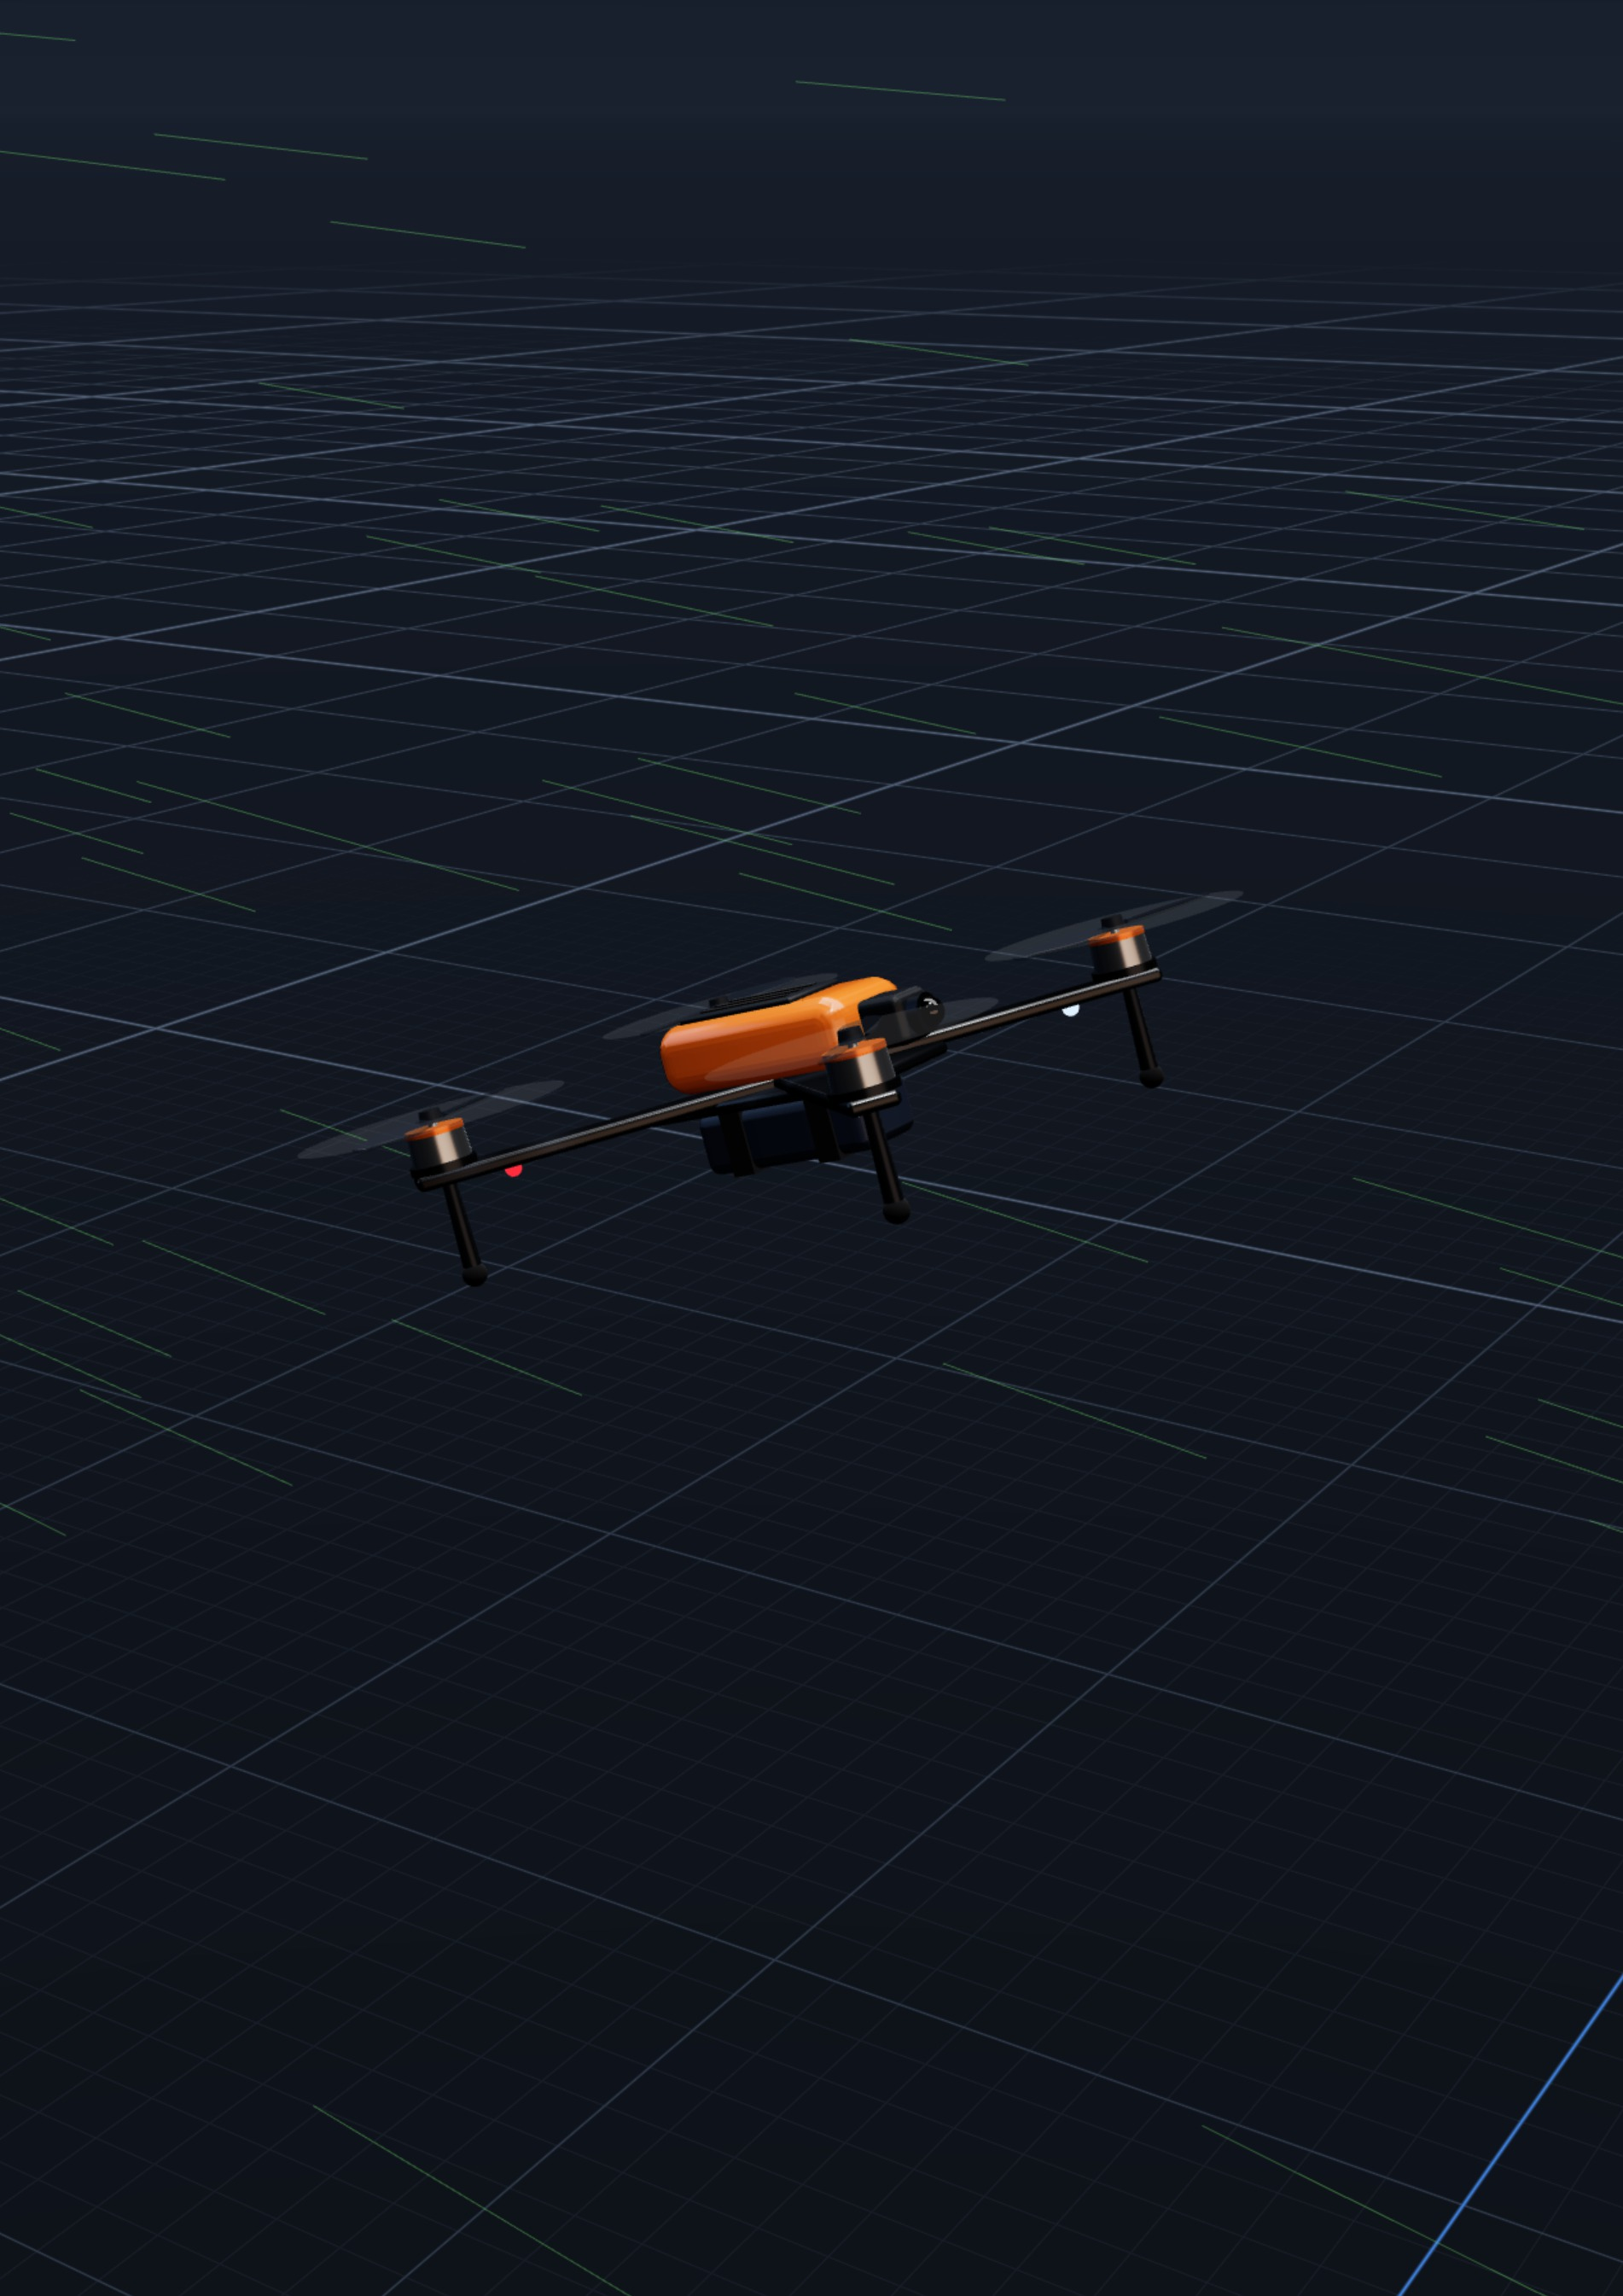
\includegraphics[width=\paperwidth, height=\paperheight]{screens/cover.jpg}};
  \fill[night, path fading=south, opacity=0.92] (current page.north west) rectangle ($(current page.north east)+(0,-120mm)$);
  \fill[night, path fading=north, opacity=0.85] ($(current page.south west)+(0,70mm)$) rectangle (current page.south east);
  \node[anchor=north west, inner sep=0pt, text=accent] at ($(current page.north west)+(24mm,-26mm)$)
    {\appmark\hspace{0.6em}\sanscaps\small A COURSE IN FEEDBACK CONTROL};
  \node[anchor=north west, inner sep=0pt, text=white, inner sep=0pt] at ($(current page.north west)+(23mm,-38mm)$)
    {\parbox[t]{170mm}{\raggedright\nohyph\sansdisplay\fontsize{54}{58}\selectfont Anemostatos}};
  \node[anchor=north west, inner sep=0pt, text=nighttext, inner sep=0pt] at ($(current page.north west)+(24mm,-64mm)$)
    {\parbox[t]{130mm}{\raggedright\displayserif\itshape\fontsize{22}{27}\selectfont Riding on the wind}};
  \node[anchor=north west, inner sep=0pt, text=nightmuted, inner sep=0pt] at ($(current page.north west)+(24mm,-78mm)$)
    {\parbox[t]{130mm}{\raggedright\sffamily\small From PID to learning, with the simulator of the same name}};
  \node[anchor=south west, inner sep=0pt, text=nightmuted, inner sep=0pt] at ($(current page.south west)+(24mm,24mm)$)
    {\parbox[b]{150mm}{\raggedright\sffamily\small The course book of the Anemostatos simulator\\[2pt]
     {\color{nightmuted!70}\footnotesize 35 lessons · 3 levels of flight · every figure flown in the simulator}\\[6pt]
     {\footnotesize Idea and editing: Wojciech Stelmaszewski · Text, figures and code: Claude Opus 5.5}}};
  \node[anchor=south east, inner sep=0pt, text=nightmuted, align=right] at ($(current page.south east)+(-18mm,24mm)$)
    {\displayserif\itshape\small ánemos + statós\\[1pt]{\sffamily\footnotesize “the one that stands in the wind”}};
\end{tikzpicture}
\null\clearpage

% ---------------------------------------------------------------- title page
\thispagestyle{empty}
\vspace*{50mm}
\noindent{\sanscaps\small\color{accent}A COURSE IN FEEDBACK CONTROL}\par\vspace{8mm}
\noindent{\sansdisplay\fontsize{36}{42}\selectfont Anemostatos}\par\vspace{5mm}
\noindent{\displayserif\itshape\fontsize{20}{25}\selectfont Riding on the wind}\par\vspace{7mm}
\noindent{\displayserif\itshape\fontsize{13}{18}\selectfont From PID to learning, with the simulator of the same name}\par
\vspace{24mm}
\noindent\begin{minipage}{118mm}\sffamily\small\color{muted}
Thirty-five lessons, each one a chapter. Every chapter explains one idea step by step, shows it in
numbers flown by the simulator, points to the exact place in the application and its source code
where the idea lives, and ends with a story of the same idea at work in the real world.
\end{minipage}
\par\vspace{16mm}
\noindent\begin{minipage}{118mm}\sffamily\small
{\color{muted}Idea and editing}\\[1pt]{\large Wojciech Stelmaszewski}\par\vspace{5mm}
{\color{muted}Text, figures and code}\\[1pt]{\large Claude Opus 5.5}
\end{minipage}
\vfill
\noindent{\sffamily\footnotesize\color{faint}Edition of 30 September 2026 · written for the simulator at commit \texttt{801cb6b} and later}
\clearpage

% ---------------------------------------------------------------- imprint ---
\thispagestyle{empty}
\vspace*{\fill}
\begin{minipage}{118mm}\sffamily\footnotesize\color{muted}\linespread{1.25}\selectfont
\textbf{\color{ink}Anemostatos: Riding on the wind} — a course in feedback control, with the simulator of the same name.\par\medskip
The idea of the course and the editing of this book are by Wojciech Stelmaszewski. The text, the figures, the
simulator and its source code were written by Claude Opus 5.5, an AI model made by Anthropic
(see the \hyperref[ch:colophon]{colophon}).\par\medskip
The simulator, its lessons and the source code referenced throughout this book live at
\url{https://github.com/wojciech-stelmaszewski/anemostatos}. Start it with \texttt{make dev}; the lesson panel on the right
of the screen follows the same numbering as this book.\par\medskip
Every time series in this book was produced by the simulator itself (\texttt{scripts/book-data.ts}), running the
same code and the same lesson set-ups as the application; the plots were drawn with \texttt{book/tools/make\_figures.py}. Screenshots
come from the running application. Photographs are public domain or under Creative Commons licences; their
authors and licences are listed on page~\pageref{credits}.\par\medskip
Set in Libertinus Serif, Libertinus Math, Fira Sans and Fira Mono with Lua\LaTeX.\par\medskip
\copyright\ 2026. Text and figures may be shared for teaching and learning.
\end{minipage}
\clearpage
